\subsection{Volume Generation}\label{subsec:Volume_Generation}
Das digitale Theremin ist auf dem Entwicklungsboard DE1-SOC von terasIC aufgebaut. Dieses enthält ein Cyclone V 5CSEMA5 FPGA von Intel. Weiter befindet sich auf dem Board der Audio Codec WM8731 von Wolfson für die Ausgabe an einem Lautsprecher. In Abbildung ... \todo{Referenz auf Blockschaltbild} ist der Aufbau des Digitalen Theremin aufgezeigt inklusive der Peripherie ausserhalb des FPGA.



\begin{figure}[h!]
	\centering
	\includegraphics[width=0.75\textwidth]{Blockschaltbild_Volume.pdf}
	\caption{Blockschaltbild der Custom IP Volume Generation} 
	\label{img:Blockschaltbild_volume}
\end{figure}  

\paragraph{Filter}

\begin{figure}[h!]
	\centering
	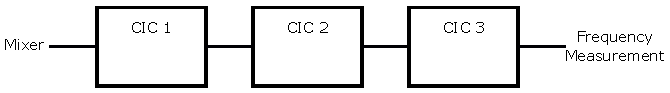
\includegraphics[width=0.8\textwidth]{Filter_volume.pdf}
	\caption{Aufbau des Filters in der Komponente Volume Generation} 
	\label{img:Filter_Volume}
\end{figure}  

\paragraph{Frequenzmessung \& Kalibration}

\begin{figure}[h!]
	\centering
	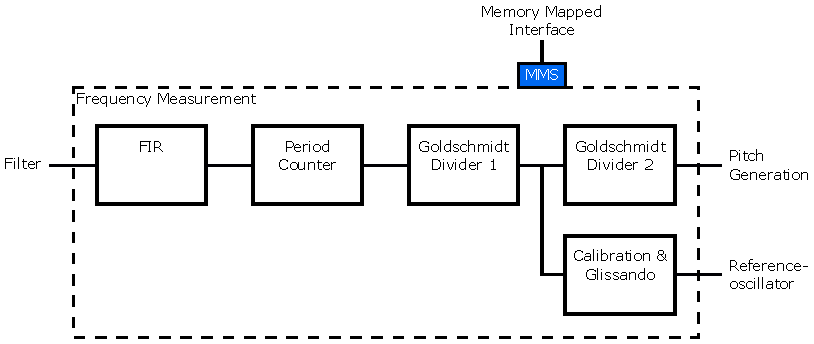
\includegraphics[width=1\textwidth]{freq_meas_volume.pdf}
	\caption{Aufbau der Frequenzmessung und Kalibration in der Komponente Volume Generation} 
	\label{img:freq_meas_volume}
\end{figure}  